\chapter{Implementation}

The main part of implementing the parser was to rewrite the EBNF provided by W3C in \cite{w3c01} to conform to ANTLR's syntax and semantics. In the following chapter we will present the reason why this was not a trivial task, the ambiguous terminals, and by which means we solved this. In addition we will present other ANTLR conforformity rewrites and finally our implementation of scoping and symbol tables.


\section{ANTLR Syntax Conformity}
The W3C(\cite{w3c00}) and ANTLR(section \ref{sect:antlr:grammarSpec}) EBNF syntax differs in multiple ways. Some of the differences are trivial, e.g. the "defined by"-operator, which in W3C syntax is denoted with \verb!::=! and in ANTLR syntax as \verb!:!. Such differences can be fixed by means of a simple symbol replacement. However, the W3C metagrammar also embodies some operators such as the 'hat' and the 'dash' operators, described in section \ref{sect:ambiguousgrammar:ambigTerm}, of which there are no complete equivalents in the ANTLR metagrammar. In addition, the W3C grammar defines some producions as terminal and other as non-terminal, but this division does not hold for all implementations.

\subsection{Seperating Parser and Lexer Rules}

The ANTLR parser generator can generate parsers and lexers from a single grammar file. The distinction between terminals and non-terminals is that terminals start with \emph{uppercase} letters, and non-terminals start with \emph{lowercase} letters. Which productions to go where is highly dependant on what strategy we chose to solve the ambigious terminals problem. E.g. by defining all the ambigious terminals as non-terminals we would have solution very close to a scan-while-parse scanner (section \ref{sect:ambiguousgrammar:scanWhileParse}). Because we chose the strategy of letting the parser control the lexer's state, we vere able define a division of terminals and non-terminals very similar to the one specified by W3C. The exception is \verb!QName!, which by W3C is defined as follows:
\begin{verbatim}
QName           ::= PrefixedName
                  | UnprefixedName
PrefixedName    ::= Prefix ':' LocalPart 
UnprefixedName  ::= LocalPart 
Prefix          ::= NCName
LocalPart       ::= NCName
\end{verbatim}
Where \verb!NCName! is another terminal, thus creating an ambiguity in the case where \verb!QName! uses the \verb!UnprefixedName! alternative. It is possible to rank the \verb!QName! production higher than the \verb!NCName! with a syntactic predicate checking if the token after \verb!NCName! is a \verb!':'!, but there is no good reason for doing so, when it can be defined as a non-terminal in this way:
\begin{verbatim}
qName             : (NCName COLONSi)? NCName;
\end{verbatim}
There is however some reasons for \emph{not} defining \verb!QName! as a terminal: by doing so, ANTLR would have generated token containing the whole \verb!QName!, meaning that e.g. if one is only interested in the localpart, one would have to manually split the text. And parser productions reffering to \verb!QName! would have to be rewritten as expecting a \verb!QName! \emph{or} a \verb!NCName!.

\subsection{Rewriting the W3C 'dash' and 'hat' operators}
The 'hat' operator (section \ref{sect:ambiguousgrammar:ambigTerm}) is mostly used to define legal characters by defining which are illigal. These productions can be rewritten in ANTLR syntax by using the not-operator ($\sim$) and a \verb!fragment! production rule \verb!NotChar! which is manually defined as all unicode characters (up to 0xFFFF, see section \ref{sect:parserconstructanddebug:limitations}) not allowed by the W3C defined \verb!Char!:
\begin{verbatim}
// The extracted part of StringLiteral:
PartOf          ::= [^"&]

// can be written in ANTLR syntax as:
PartOf            : ~(NotChar | COLONSi | AMPSi);
\end{verbatim}
The 'dash' operator is sometimes also used like this, like in e.g. \verb!QuotAttrContentChar! but because of our introduced production \verb!QuotAttributeContent! (section \ref{sect:rewriteGrammar:introduceStates}) it is rewritten in the same way as with the enclosed expressions (section \ref{sect:rewriteGrammar:enclosedComposite}), where the operator is used to define that a very gereral production should not be greedy. 

In \verb!piTarget! the 'dash' operator is used in a unique way, and thus needed to be treated differently:
\begin{verbatim}
// Original production
PiTarget    ::= Name - (('X' | 'x') ('M' | 'm') ('L' | 'l'))

// Rewritten production using a semantic predicate
piTarget    : n=Name { !$n.getText().equalsIgnoreCase("XML") }?;
\end{verbatim}
Where the original production can be interpreted as ``piTarget can be a Name, but not `XML', regardless of character casing''. The validating semantic predicate will imitate this behaviour using the method \verb!equalsIgnoreCase()!.

\section{Parser Controlled State Driven Lexer}
As we saw in section \ref{sect:ambiguousgrammar:ambigTerm}, unless we employ a scan-while-parse scanning strategy, we need to make the lexer somehow aware of the context of incomming characters to be able to correctly generate tokens. Our parser controlled state driven lexer strategy implies that the parser must directly infulence the state of the lexer, and the lexer must know what state it is in \emph{before} trying to match a token. 

ANTLRs default parser input \verb!TokenStream!, \verb!CommonTokenStream!, will at first peek ask the lexer to generate tokens until \verb!EOF! and place them in a buffer, meaning that the parser will be in an initial state as the lexer runs. This is not compatible with our lexer strategy, so we had to make our own \verb!TokenStream!, not buffering more than strictly needed. This method as well as how we control the state transitions, how we introduced container tokens to ease the parsing and how we reorganized the grammar to make it susceptible to states will be discussed in the following sections.

\subsection{UnbufferedCommonTokenStream}
For an overview of how the lexer, parser and tokenen stream is connected see section \ref{sect:antlr:parser}. ANTLRs \verb!CommonTokenStream! has a method \verb!LT(int k)! which returns the $k$th token forward from its current position (simplified):
\begin{verbatim}
public Token LT(int k) {
      if ( p == -1 ) {
         fillBuffer();
      }
      int i = p;
      int n = 1;
      while ( n<k ) {
         i = skipOffTokenChannels(i+1); // leave p on valid token
         n++;
      }
      if ( i>=tokens.size() ) {
         return Token.EOF_TOKEN;
      }
      return (Token)tokens.get(i);
}
\end{verbatim}
Where \verb!p! a pointer to the current token in the token stream, \verb!tokens! is a list of the tokens generated, and the method \verb!skipOffTokenChannels(int r)! returns the position number bigger or equal to \verb!r! on which there resides a valid token, i.e. a token in the default virtual channel (identified by the integer \verb!channel!). The pionter \verb!p! is initialized to $-1$, thus the the first time \verb!LT(int k)! is run, it calls method \verb!fillBuffer()! (simplified):
\begin{verbatim}
protected void fillBuffer() {
   Token t = tokenSource.nextToken();
   while ( t!=null && t.getType()!=CharStream.EOF ) {
      tokens.add(t);
      t = tokenSource.nextToken();
   }
   p = skipOffTokenChannels(0);
}
\end{verbatim}
Where \verb!tokenSource! is the lexer connected. The omitted parts of the code are mainly related to virtual channel handling and other means to hide tokens from the parser. Both of these methods had to be overridden in our \verb!CommonTokenStream! derived \verb!UnbufferedCommonTokenStream!. The name \verb!UnbufferedCommonTokenStream! can be a bit misleading, as it does buffer all allready matched tokens -- but only as many tokens forward as necessary at any given time. To implement this we introduced a method \verb!fillBuffer(int k)! which fills the buffer with $k$ new \emph{valid} tokens (simplified):
\begin{verbatim}
protected void fillBuffer(int k) 
{
   int no = 0;
   Token t = tokenSource.nextToken();
   while (t!=null && t.getType()!=CharStream.EOF) 
   {
      t.setTokenIndex(tokenIndex);
      tokens.add(t);
      tokenIndex++;
      if(t.getChannel()==channel)
         if(++no == k){
            p = skipOffTokenChannels(p);
            break;
         }
      t = tokenSource.nextToken();
   }
}
\end{verbatim}
Where \verb!channel! identifies the valid virtual channel, and the \verb!no! variable acts as a valid tokens encountered counter. The pointer \verb!p! must be adjusted right before \verb!break! to ensure that does not point to a hidden token. A filling of the buffer such as this, though, must only take place when there are not enough tokens generated, This lead us to insert a check in our overridden \verb!LT(int k)!, which we implemented in form of a method \verb!enoughValidLH(int k)!:
\begin{verbatim}
protected boolean enoughValidLH(int k)
{
   int i = p;
   int n = tokens.size();
   int no = 0;
   while (i<n) {
      if(((Token)tokens.get(i)).getChannel()==channel)
         if(++no == k)
            return true;
         i++;
      }
   return false;
}
\end{verbatim}
Where \verb!no! once again acts as a counter over valid tokens. The \verb!while! construct til iterate until enough such tokens are identified, or it reaches the end of the buffer.

\subsection{Introducing the States}
\label{sect:rewriteGrammar:introduceStates}
Looking at the ambiguous terminals in section \ref{sect:ambiguousgrammar:ambigTerm} we found that we would need to differenciate between \verb!ElementContentChar!, \verb!QuotAttrContentChar! and \verb!AposAttrContentChar!, and between these these productions and all the other productions. In addition would the overlap between \verb!DirAttributeValue! and \verb!StringLitteral! be addressed. Figure \ref{fig:ambigTerminalRef} shows where these productions are referred to (or not referred to in the case of \verb!StringLitteral!) in the W3C specified grammar. As we can see, neither of the problem terminals are ambigious when enclosed in higher level productions -- a necessity for our state driven strategy. We also see that all the problem terminals are in a way connected to XML markup, and consist of the characters allowed as the text in elements and the characters allowed as attribute values.
\begin{figure}[h]
\begin{verbatim}
DirElemConst    ::= "<" QName DirAttributeList 
                      ("/>" 
                     |(">" DirElemContent* "</" QName ">")
                      )
DirAttrList     ::= (QName "=" DirAttrValue)*
DirAttrValue    ::= ('"' (EscapeQuot|QuotAttrValCont)* '"')
                  | ("'"(EscapeApos|AposAttrValCont)* "'")
QuotAttrValCont ::= QuotAttrContentChar
                  | CommonContent
AposAttrValCont ::= AposAttrContentChar
                  | CommonContent
DirElemContent  ::= ElementContentChar
                  | CommonContent
CommonContent   ::= "{{" | "}}" | EnclosedExpr
EnclosedExpr    ::= "{" Expr "}"
\end{verbatim}
\caption[Grammar reffering to amiguous terminals.]{A simplified overview of the non-terminal productions refering to the ambiguous terminals. \textbf{EscapeApos} is \textbf{''} and is used to escape the single \textbf{'} within a apostrophe enveloped construct, and the analog for the quote sign \textbf{"} is \textbf{EscapeQuot}. \textbf{Expr} is a very high-level production able to match almost any legal XQuery syntax.}
\label{fig:ambigTerminalRef}
\end{figure}
Explained with an example input character stream, \verb!<a id="1" z='2'>b</a>!, and where \framebox[1.0\width]{$\times$} marks the spot where the lexer is in the respective state, our five defined states are shown in figure \ref{fig:states}.
\begin{figure}[h]
\centering
\begin{tabular}{ll}
DEFAULT				& \framebox[1.0\width]{$\times$}\verb!<a id="1" z='2'>b</a>!\framebox[1.0\width]{$\times$} \\
IN\_TAG				& \verb!<!\framebox[1.0\width]{\texttt{a}}\verb! id="1" z='2'>b</a>! \\
IN\_APOS\_ATTRIBUTE\verb!   !	& \verb!<a id="1" z='!\framebox[1.0\width]{\texttt{2}}\verb!'>b</a>! \\
IN\_QUOT\_ATTRIBUTE		& \verb!<a id="!\framebox[1.0\width]{\texttt{1}}\verb!" z='2'>b</a>! \\
IN\_ELEMENT			& \verb!<a id="1" z='2'>!\framebox[1.0\width]{\texttt{b}}\verb!</a>! \\
\end{tabular}
\caption{An illustrated overview of the different states.}
\label{fig:states}
\end{figure}


\textbf{\LARGE //TODO:} 

ElementContent, Apossoppassellers etc..



\subsection{State Transitions}


\textbf{\LARGE //TODO:} 

Hvordan parseren gaar over fra en state til en annen, systemet med stack.

\subsection{Reorganizing the Grammar}
\label{sect:rewriteGrammar:reorganizing}
\textbf{\LARGE //TODO:} 

Slik at state-systemet fungerer: Lage fragment av alt, TOKENSWITCH, semantiske predikat, etc.


\section{Enclosed Composite Lexer Productions}
\label{sect:rewriteGrammar:enclosedComposite}
\textbf{\LARGE //TODO:} 

Regler som PI, Pragma, XMLComment and CDATA kan fanges i sin helhet i lexeren. Samme med saertilfellet XQuerykommentarer. 

Fint for aa skille alternativer, men man ikke faar tak i deltokens... saa derfor ----v

\subsection{Emiting More Than One Token Per Production}
\textbf{\LARGE //TODO:} 

Omskriving av lexer for a la produksjoner avgi mer enn ett token

\subsection{PI, Pragma, XMLComment and CDATA Sections}
\textbf{\LARGE //TODO:} 

Sammensatte omhyllede lexerregler (<? noe ?>, <!-- noe --> etc)

\subsection{Nested XQuery Comments}
XQuery allows nested comments, for example:
\begin{verbatim}
(: this is a comment (: this comment is nested :) :)
\end{verbatim}
This is a classic problem in compiler construction, however it can be solved using standard ANTLR syntax, without resorting to custom functions/methods for consuming input and keeping track of nesting. The original EBNF as specified by W3C is as follows:
\begin{verbatim}
Comment ::= "(:" (CommentContents | Comment)* ":)"
\end{verbatim}
At first glance, this seems uncomplicated and straight forward, but this grammar needs to be rewritten to be accepted by an LL parser. A suggestion for a solution to this problem was initially found on the Antlr mailing list\footnote{http://www.antlr.org:8080/pipermail/antlr-interest/2005-July/012967.html}, and we loosly based our implementation on such an approach. This lexer rule will correctly detect and allow nested comments, and hide them from the parser:
\begin{verbatim}   
Comment   : LXQCOMMENTSi 
           ({(input.LA(1)=='(' && input.LA(2)==':')}?Comment 
           | {input.LA(2)!=')'}?=>COLONSi
           | {input.LA(2)!=':'}?=>LPARSi
           | ~(LPARSi | COLONSi | NotChar))*
            RXQCOMMENTSi; {$channel=HIDDEN;}
    fragment LXQCOMMENTSi     : '(:';
    fragment RXQCOMMENTSi     : ':)';
\end{verbatim}
Where the disambiguating semantic predicate on the second line can be understood as "if it looks like a comment, it is a comment". The gated semantic predicates on the third and fourth line guards the production from being greedy, i.e. they hide the posibility of matching a \verb!':'! if it is followed by a \verb!')'!, and \verb!'('! if it is followed by a \verb!':'!. By using \verb!$channel=HIDDEN! ANTLR will put this token in an different virtual channel than the default one, making it invisible for the parser unless explicitly asked for. 

\section{Differentiating NCName and Keywords}

\textbf{\LARGE //TODO:} 

Systemet med NCNames vs keywords. \\
Husk: Keywords er uttrykt som tokens for aa sperre av for parsing og for oversiktlige feilmeldinger.

\section{Extra-grammatical Constraints}

\textbf{\LARGE //TODO:} 

Whitespace, leading dash etc..

\section{Resolving Non-determinisms in the Parser }

\textbf{\LARGE //TODO:} 

pathExpr og itemtype occurenceindicator trengte syntaktiske predikat

\section{Reserved Keywords}

\underline{\textbf{\LARGE //TODO:}} dette maa flyttes eller skrives om.

A particular feature in XQuery is the lack of reserved keywords. This creates a
series of problems when a lexer based on the verbatim grammar specification from
the W3C is trying to recognize tokens. 

vaar parser har enna reserved keywords, flytte dette til future work? \\
\underline{\textbf{\LARGE //ODOT:}} 




\section{Scoping and symbol tables}
Scoping was implemented using a simple tree structure consisting of parent- and
child scopes. XQuery only allows new scopes to be defined through the
enclosedExpr production rule. This makes it trivial to start a new scope at the
beginning of a enclosedExpr, and end the scope and the end of an enclosedExpr.
This has been implemented as follows:
\begin{figure}[!h]
\begin{verbatim}
enclosedExpr : 
    LBRACESi {
        Scope parent = this.currentScope; 
        this.currentScope = new Scope(); 
        this.currentScope.setParent(parent); 
    }
    expr 
    RBRACSi { 
        this.currentScope = this.currentScope.getParent(); 
    }
;
\end{verbatim}
\caption{Scoping logic embedded in grammar definition}
\end{figure}

Where this.currentScope is a reference to the ``current'' scope in this
context. This member variable is initiated with an empty scope when an object
of the parser class is instantiated.

The implementation above (which is formatted slightly for brevity) will
automatically build a scope tree as the input is parsed.

The currentScope object, which is an object of type Scope, holds one reference
to a symbol table. The symbol table, which is a simple subclass of
java.util.HashMap, is not capable of performing symbol lookups throughout the
scope tree. This functionality is rather provided by the Scope class. This UML diagram
illustrates the relationship between the Scope, SymTab, and Symbol classes:
\clearpage
\begin{figure}[!h]
  \centering
    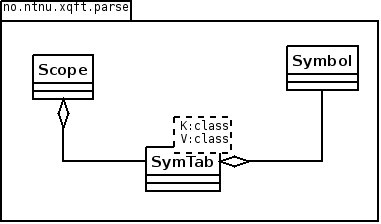
\includegraphics[scale=0.8]{img/uml1}
  \caption{Simplified UML overview of classes related to scope and symbol table}
\end{figure}

\section{Type checking}
XQuery/XPath has a well-defined type hierarchy.
\begin{figure}[h!]
  \centering
    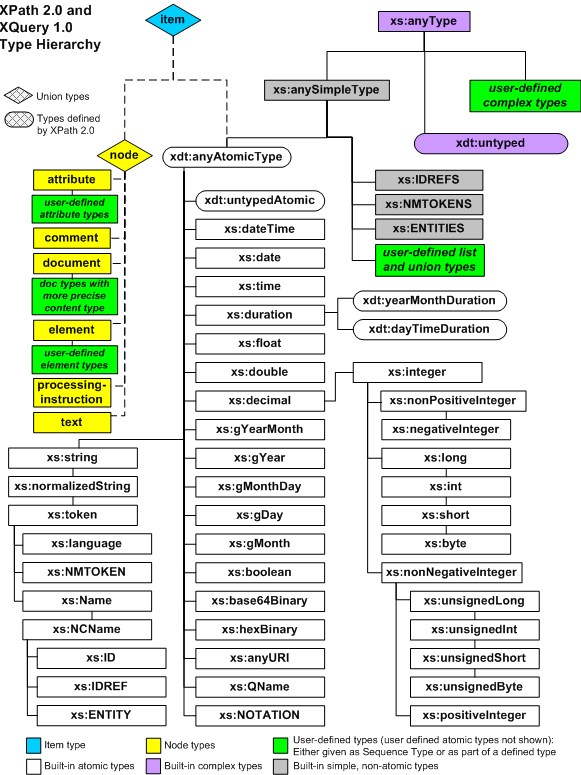
\includegraphics[scale=0.5]{img/xpathtypehierarchy}
  \caption{XQuery/XPath type hierarchy \cite{w3c04} (copyright
  \copyright W3C)}
\end{figure}
Here is a short overview of the basic type system:
\begin{itemize}
  \item Node types
    \begin{itemize}
      \item element()
      \item attribute()
      \item text()
      \item commment()
      \item document-node()
      \item processing-instruction()
    \end{itemize}
  \item Structure types
    \begin{itemize}
      \item Atomic types (xs:integer, xs:string, ..)
      \item Simple types (list, union)
      \item Complex types (user-defined types from an XML schema, except
      xs:anyType and xdt:untyped)
    \end{itemize}
\end{itemize}

Atomic types are strongly typed except xs:untypedAtomic, xs:anyURI, as well as
numerical types (xs:integer, xs:double, ..). Non-atomic simple types as well as
complex types are both strongly typed.

Proper type checking requires implementation of type inference and type
synthesis. This requires a stable abstract syntax tree and advanced data flow
analysis techniques to be feasible. Due to the inherent limitations in this
project, type checking has not been implemented - however the possibility of
this is discussed in section \ref{sect:summary:future_work}.

\underline{\textbf{\LARGE //TODO:}}
\begin{itemize}
  \item Dynamic vs. Static typing
  \item Strong vs. Weak (what and when)
  \item Type inference
  \item Michael Rys
\end{itemize}

\underline{\textbf{\LARGE //ODOT:}}

\section{TODO}

\underline{\textbf{\LARGE //TODO:}}
\begin{itemize}
\item Sammensatte omhyllede lexerregler (<? noe ?>, <!-- noe --> etc)
\item Omskriving av lexer for a la produksjoner avgi mer enn ett token
\item Omskriving av TokenStream for at den ikke skal buffre mer en strengt tatt nodvendig
\item Kjempetvetydigheten med ElementContentChar / AttributeContentChar / NCName etc.
\item Systemet med states, stack og parser snakker direkte til lexer
\item Systemet med NCNames vs keywords
\end{itemize}

\underline{\textbf{\LARGE //ODOT:}}